% ======================================================================
\subsection{FC3 decomposition for the NEGF self-energy}
\label{sub:pcp_analysis}
% ======================================================================

This subsection analyzes FC3 decomposition strategies for the
phonon-phonon self-energy in the NEGF framework.  The separable (SVD)
decomposition is the recommended approach: it converges systematically
to the dense result and preserves matrix structure through the
frequency convolution.

We first present the SVD approximation quality
(\cref{sssub:pcp_quality}), cost analysis (\cref{sssub:cost_analysis}),
and thickness-dependent validation (\cref{sssub:thickness_validation}).
\Cref{sssub:scba_investigation} investigates SCBA convergence limits
using a toy model and FC3/FC2 strength analysis.
\Cref{sssub:svd_asr} evaluates ASR enforcement,
\cref{sssub:pcp_note} explains why rank-1 (PCP) decompositions fail
for NEGF, and \cref{sssub:tensor_decomp} surveys tensor decomposition
strategies for future improvements.


% -------------------------------------------------------
\subsubsection{Approximation quality}
\label{sssub:pcp_quality}
% -------------------------------------------------------

All results in this section use the Si $2\times 2\times 2$ test case
with a $4\times 4$ $q$-mesh, 101 frequency points from
1.0--14.0\,THz, up to 10 SCBA iterations (tol.\ 0.5\%), and mixing
0.3.  The dense reference gives
$G_\mathrm{anh} = 827\,\mathrm{MW/(m^2\,K)}$.

\paragraph{FC3 reconstruction error.}
\Cref{fig:fc3_error} shows the singular value spectrum of the
stacked FC3 matrix (left) and the reconstruction error vs.\ SVD
rank (right).  The error decreases monotonically by construction,
reaching $< 3\%$ at $R = 12$ and machine precision at $R = 24$
(the full rank).

\begin{figure}[htbp]
  \centering
  \includegraphics[width=\textwidth]{figures/fc3_error_vs_rank.pdf}
  \caption{(a) Singular value spectrum of the stacked FC3 matrix.
    (b) FC3 reconstruction error vs.\ SVD rank.}
  \label{fig:fc3_error}
\end{figure}

\paragraph{Transport accuracy vs.\ rank.}
\Cref{fig:transport_rank} shows $G_\mathrm{anh}$ and the relative
transport error as a function of SVD rank.  The separable
approximation converges monotonically to the dense result, reaching
$< 1\%$ error at $R = 12$ and matching dense exactly at $R = 24$.

\begin{figure}[htbp]
  \centering
  \includegraphics[width=\textwidth]{figures/transport_vs_rank.pdf}
  \caption{(a) Thermal conductance $G_\mathrm{anh}$ vs.\ SVD rank.
    The separable result (green) converges to the dense reference
    (red line).
    (b) Relative transport error.  The green band marks the $\pm 5\%$
    region; SVD enters this band at $R \geq 6$.}
  \label{fig:transport_rank}
\end{figure}

\begin{table}[h]
\centering
\caption{Transport results for Si 300\,K.  Dense reference:
$G_\mathrm{anh} = 827\,\mathrm{MW/(m^2\,K)}$.}
\label{tab:accuracy}
\begin{tabular}{lccccc}
  \toprule
  Method & FC3 err. & $G_\mathrm{anh}$ [MW] & Transp.\ err.
         & Conserv. & Time [s] \\
  \midrule
  Dense           & ---     & 827  & ---       & 2.8\% & 53 \\
  SVD $R=2$       & 43.3\%  & 1054 & $+27.5\%$ & 0.4\% & 4 \\
  SVD $R=4$       & 22.2\%  & 957  & $+15.7\%$ & 1.2\% & 20 \\
  SVD $R=6$       & 12.3\%  & 848  & $+2.5\%$  & 2.5\% & 22 \\
  SVD $R=12$      & 2.8\%   & 831  & $+0.4\%$  & 2.8\% & 31 \\
  SVD $R=24$      & 0.1\%   & 827  & $-0.0\%$  & 2.8\% & 47 \\
  \bottomrule
\end{tabular}
\end{table}

\paragraph{Spectral heat current.}
\Cref{fig:spectral_current} shows the frequency-resolved heat
current (left) and its deviation from the dense reference (right).
SVD $R = 6$ deviates mostly at the acoustic peak ($\sim 4$\,THz) but
tracks dense closely elsewhere.  SVD $R = 24$ is indistinguishable
from dense.

\begin{figure}[htbp]
  \centering
  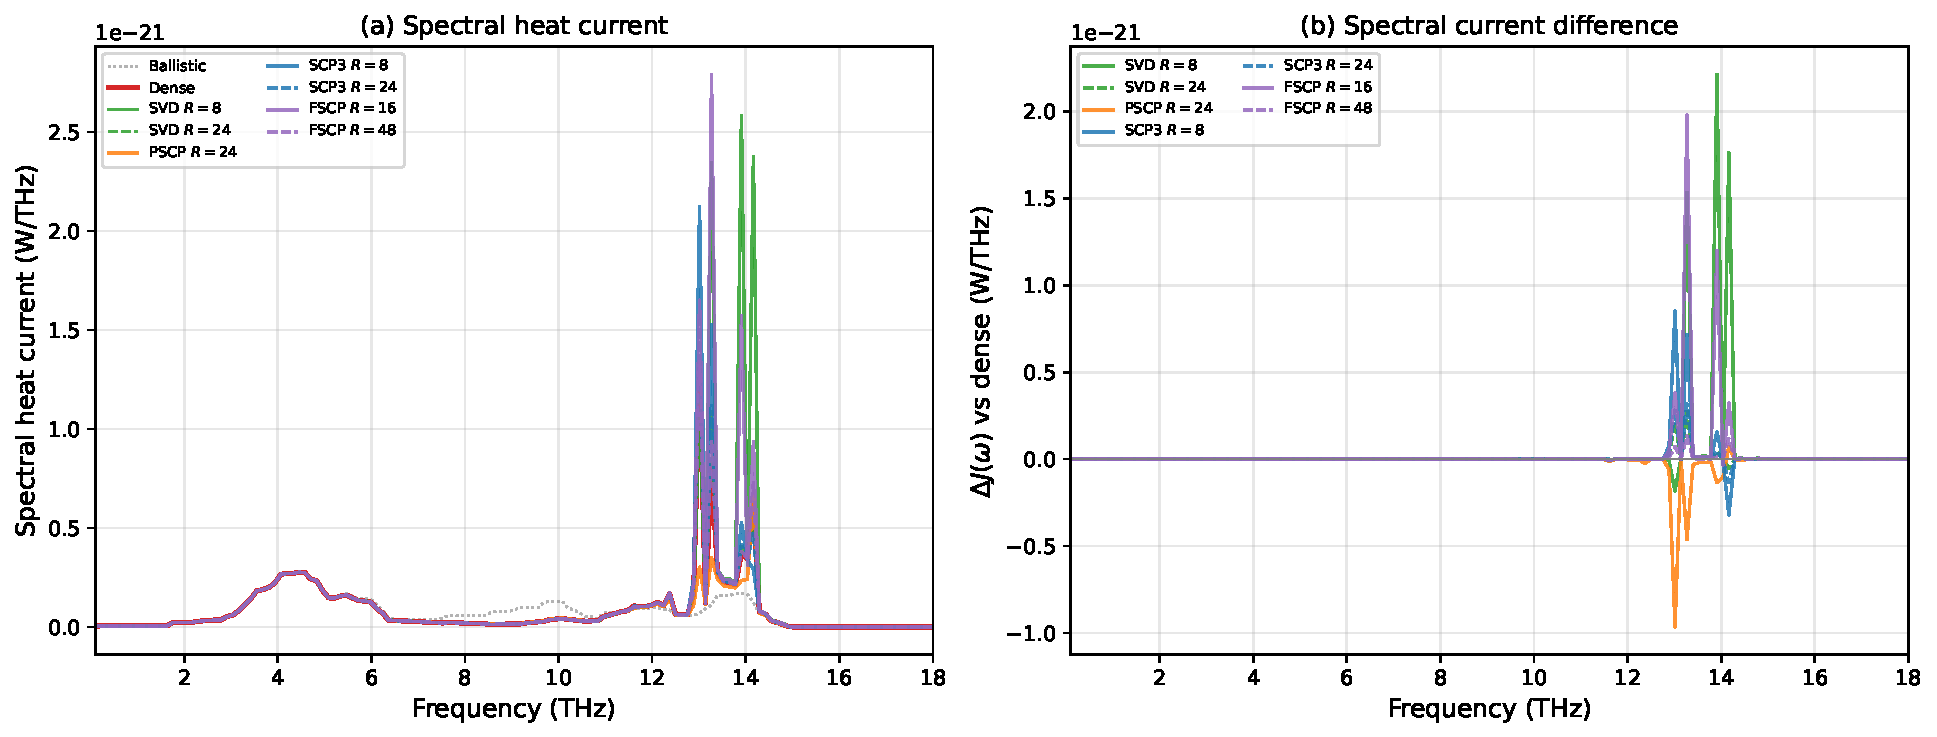
\includegraphics[width=\textwidth]{figures/spectral_current.pdf}
  \caption{(a) Spectral heat current for selected methods.
    (b) Difference from dense: SVD $R = 24$ is indistinguishable from
    dense; SVD $R = 6$ shows small deviations near the acoustic peak.}
  \label{fig:spectral_current}
\end{figure}

\paragraph{Self-energy comparison.}
\Cref{fig:sigma_compare} shows the phonon broadening
$-\mathrm{Tr}[\mathrm{Im}\,\Sigma^R]/M$ (left) and the relative
Frobenius error of the self-energy vs.\ frequency (right).
SVD $R = 24$ reproduces the dense self-energy to $< 1\%$ at all
frequencies.

\begin{figure}[htbp]
  \centering
  \includegraphics[width=\textwidth]{figures/self_energy_comparison.pdf}
  \caption{(a) Phonon broadening (q-averaged).
    (b) Relative Frobenius error of the self-energy vs.\ frequency.
    SVD converges systematically with increasing rank.}
  \label{fig:sigma_compare}
\end{figure}

\paragraph{FC3 error vs.\ transport error.}
\Cref{fig:error_decomp} plots the FC3 reconstruction error against
the transport error.  SVD points follow the
$\epsilon_G \approx \delta_\Phi$ line: transport error is directly
proportional to the FC3 truncation error, confirming that no
structural error is introduced by the decomposition.

\begin{figure}[htbp]
  \centering
  \includegraphics[width=0.7\textwidth]{figures/error_decomposition.pdf}
  \caption{FC3 reconstruction error vs.\ transport error.
    SVD (green squares) follows $\epsilon_G \propto \delta_\Phi$:
    better FC3 $\Rightarrow$ better transport.}
  \label{fig:error_decomp}
\end{figure}

\paragraph{Conservation and cost trade-off.}
\Cref{fig:conserv_pareto} shows conservation error (left) and the
accuracy--cost Pareto front (right).  SVD $R = 6$ (22\,s, 2.5\%
error) and SVD $R = 12$ (31\,s, 0.4\% error) provide excellent
accuracy--cost trade-offs.

\begin{figure}[htbp]
  \centering
  \includegraphics[width=\textwidth]{figures/conservation_and_timing.pdf}
  \caption{(a) Heat flow conservation error.
    (b) Pareto front: $G_\mathrm{anh}$ accuracy vs.\ wall time.
    The green band marks $\pm 5\%$ of the dense reference.}
  \label{fig:conserv_pareto}
\end{figure}

\paragraph{SCBA convergence.}
\Cref{fig:scba_conv} shows the SCBA convergence behaviour.  All
SVD ranks converge at similar rates, requiring $\sim$10 iterations.
Low-rank cases ($R = 2$) converge slightly faster because their
stronger FC3 approximation produces smaller self-energies.

\begin{figure}[htbp]
  \centering
  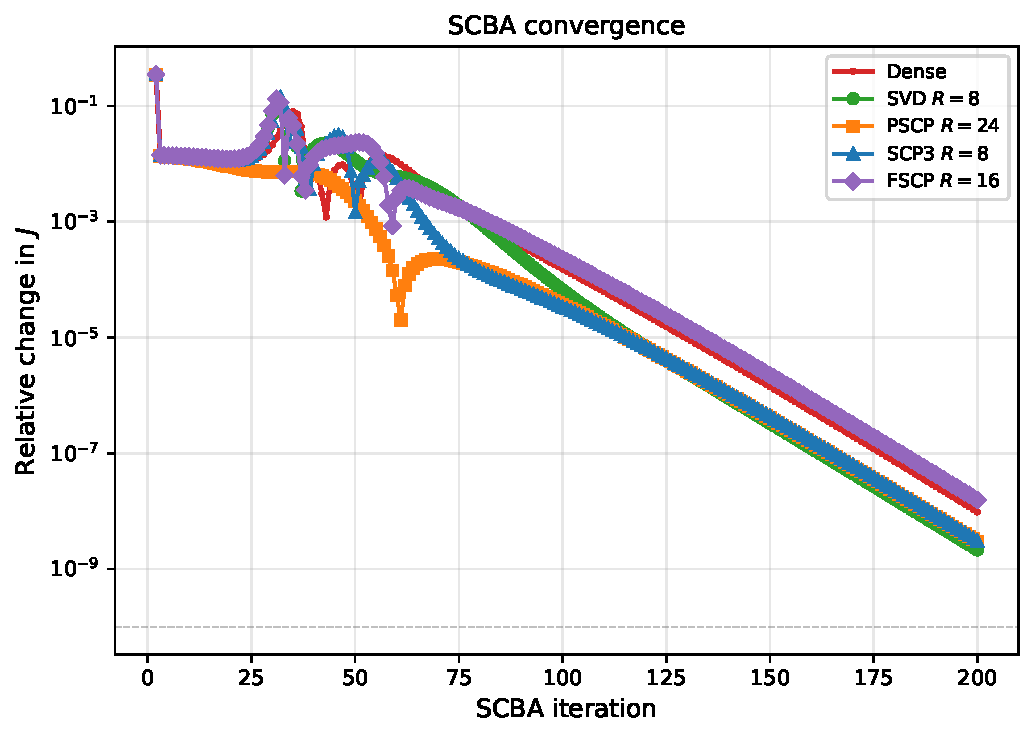
\includegraphics[width=\textwidth]{figures/scba_convergence.pdf}
  \caption{(a) SCBA convergence: relative change in total heat
    current vs.\ iteration.
    (b) Total iterations to convergence.}
  \label{fig:scba_conv}
\end{figure}

\paragraph{Key findings.}
\begin{enumerate}
  \item \textbf{SVD converges systematically}: transport error
    decreases monotonically with rank, reaching $< 1\%$ at $R = 12$.
  \item \textbf{No structural error}: the FC3--transport error
    relationship follows $\epsilon_G \propto \delta_\Phi$, confirming
    that only the FC3 truncation contributes to transport error.
  \item \textbf{$R = 6$ is practical}: 2.5\% transport error at
    $2.4\times$ speedup over dense makes $R = 6$ the recommended
    default for Si-scale cells.
  \item \textbf{$R = 12$ is high-accuracy}: 0.4\% error at
    $1.7\times$ speedup for applications requiring reference-quality
    results.
\end{enumerate}


% -------------------------------------------------------
\subsubsection{Cost analysis}
\label{sssub:cost_analysis}
% -------------------------------------------------------

The separable kernel replaces the dense per-pair cost with a sum
over $R^2$ rank pairs.  For each $(\vq,\vq')$ pair:
\begin{equation}\label{eq:sep_cost}
  \cW_\mathrm{sep}^{\mathrm{pair}}
  = \underbrace{R^2\,N_\tau \log N_\tau}_{\text{batch IFFT}}
  + \underbrace{R^2\,N_\omega\,M^2}_{\text{accumulation}},
\end{equation}
where $M = n_\mathrm{dof} = 6$ for Si.  The dense kernel has cost
\begin{equation}
  \cW_\mathrm{dense}^{\mathrm{pair}}
  = M^4\,N_\tau \log N_\tau + N_\omega\,(M^5 + M^4).
\end{equation}
The separable kernel is faster when $R^2 < M^4$, i.e., $R < M^2$.
For Si ($M = 6$): at $R = 6$, $R^2 = 36 \ll M^4 = 1296$, giving
$\sim 36\times$ fewer IFFT operations.

\paragraph{Measured per-pair timings (Si, $M = 6$, one channel).}
\begin{center}
\begin{tabular}{lrrr}
  \toprule
  Method & Cost/pair (ms) & $\times N_q^2 \times 2$ (s) & vs.\ dense \\
  \midrule
  Dense             & 8.7  & 4.5  & $1.0\times$ \\
  Separable $R=6$   & 2.3  & 1.2  & $3.8\times$ faster \\
  Separable $R=12$  & 3.8  & 1.9  & $2.3\times$ faster \\
  Separable $R=24$  & 8.5  & 4.4  & $1.0\times$ \\
  \bottomrule
\end{tabular}
\end{center}

\paragraph{Scaling with primitive cell size.}
The dense kernel scales as $M^4$--$M^5$ per pair, while the separable
kernel scales as $M^2 R^2$ (accumulation-dominated for large $M$).
\Cref{fig:sep_R} shows the separable per-pair cost vs.\ rank for
different cell sizes.  At $M = 48$ (16-atom cell), even $R = 6$ costs
4.5\,s per pair---comparable to dense---because the $M^2$ accumulation
dominates.  This motivates the Tucker decomposition discussed in
\cref{sssub:tensor_decomp}, which can reduce the $M^2$ factor to
$r_1^2$ with $r_1 \ll M$.

\begin{figure}[htbp]
  \centering
  \includegraphics[width=0.7\textwidth]{figures/sep_scaling_R.pdf}
  \caption{Separable per-pair cost vs.\ SVD rank $R$ for different
    cell sizes.  At $M = 48$, even $R = 6$ costs 4.5\,s---comparable to
    dense---because the $M^2$ accumulation dominates.}
  \label{fig:sep_R}
\end{figure}

For the Si test case ($M = 6$), the optimal operating point is
$R = 6$--$12$: the per-pair cost is $3$--$4\times$ cheaper than dense,
while the total SCBA wall time (including overhead for SVD decomposition
and Fourier transforms) gives $1.7$--$2.4\times$ end-to-end speedup
(\cref{tab:accuracy}).


% -------------------------------------------------------
\subsubsection{Thickness-dependent thermal conductivity}
\label{sssub:thickness_validation}
% -------------------------------------------------------

To validate the separable kernel on a physically meaningful benchmark,
we reproduce the thickness-dependent cross-plane thermal conductivity
of a silicon thin film at 300\,K, following Guo et~al.\
\cite{guo_quantum_2020}.  The setup models a thin film of thickness~$d$
between two semi-infinite Si contacts, with a temperature difference
$\Delta T = 10$\,K.  The thermal conductivity is computed as
$\kappa_\mathrm{eff} = G \cdot d$, where $G = J / (A_c \Delta T)$ is
the thermal conductance and $d = n_\mathrm{slabs} \times a/2$ is the
film thickness (one FCC primitive cell per slab, $a/2 = 2.73$\,\AA{}
along~$[100]$).

\Cref{fig:thickness_kappa} shows the thickness-dependent thermal
conductivity computed with the separable kernel ($R = 12$, $4 \times 4$
$q$-mesh, 101 frequency points, 0.5--15.5\,THz).  Both the ballistic
and anharmonic results are compared with the data of
Guo et~al.\ (first nearest-neighbor FC3, DFT input).

\begin{figure}[htbp]
  \centering
  \includegraphics[width=\textwidth]{figures/thickness_conductivity.pdf}
  \caption{(a) Cross-plane thermal conductivity of a Si thin film at
    300\,K vs.\ thickness, computed with the separable kernel
    ($R = 12$) and compared with Guo et~al.\ \cite{guo_quantum_2020}.
    Open symbols: reference data; filled symbols: present work.
    (b) Thermal conductance vs.\ thickness, showing the ballistic
    (circles) and anharmonic (triangles) results.}
  \label{fig:thickness_kappa}
\end{figure}

The anharmonic reduction of thermal conductivity increases with film
thickness, as expected: thicker films allow more phonon-phonon
scattering.  The SCBA converges reliably up to $n_\mathrm{slabs} = 6$
($d \approx 1.6$\,nm).  At $n_\mathrm{slabs} = 10$, the solver
terminates but yields 47.8\% conservation error---this point is
unconverged and should be treated with caution (see
\cref{sssub:scba_investigation} for a detailed convergence analysis).
For the converged data points ($n_\mathrm{slabs} \leq 6$), the
anharmonic reduction is 30--50\%, qualitatively consistent with
Guo et~al.\ but quantitatively larger due to our smaller FC3
supercell ($2\times 2\times 2$ vs.\ $3\times 3\times 3$).

\Cref{fig:thickness_spectral} shows the spectral heat current at
different thicknesses, illustrating how anharmonic scattering
redistributes spectral weight from acoustic modes ($\sim$2--5\,THz)
to optical modes ($\sim$8--14\,THz) with increasing film thickness.

\begin{figure}[htbp]
  \centering
  \includegraphics[width=\textwidth]{figures/thickness_spectral.pdf}
  \caption{(a) Spectral heat current vs.\ frequency for different
    film thicknesses (solid: anharmonic, dashed: ballistic).
    (b) Anharmonic conductance reduction vs.\ thickness.}
  \label{fig:thickness_spectral}
\end{figure}


% -------------------------------------------------------
\subsubsection{SCBA convergence investigation}
\label{sssub:scba_investigation}
% -------------------------------------------------------

The thickness sweep of \cref{sssub:thickness_validation} reveals that
the SCBA diverges for thicknesses above $\sim$6 primitive slabs
($\gtrsim 1.6$\,nm), even with reduced mixing parameters.  This
section investigates the root cause by (a) validating the solver
equations with a toy model, (b) quantifying the anharmonic coupling
strength ratio FC3/FC2, and (c) identifying the physical regime in
which the perturbative SCBA is valid.

\paragraph{Toy model validation.}
To distinguish solver bugs from physical convergence limits, we
construct a synthetic simple-cubic crystal with one atom per cell
($a = 3$\,\AA, $m = 28$\,amu), nearest-neighbor harmonic springs
($k = 5$\,eV/\AA$^2$), and nearest-neighbor cubic anharmonicity
($\Phi_3$, isotropic, fully $S_3$-symmetrized).  This model is fed
through the \emph{existing} separable SCBA code---no equations are
reimplemented.  \Cref{tab:toy_weak} shows that for weak anharmonicity
($\Phi_3 = 0.5$\,eV/\AA$^3$), the SCBA converges at all tested device
thicknesses ($n_\mathrm{slabs} = 1$--$10$) with heat-flow conservation
$<$3.8\% and physical conductance reduction with increasing thickness.
This confirms the solver implementation is correct.

\begin{table}[h]
  \centering
  \caption{SCBA convergence for the toy model with weak anharmonicity
    ($\Phi_3 = 0.5$\,eV/\AA$^3$, $\alpha = 0.001$).
    All runs use $2\times 2$ $q$-mesh and mixing~0.3.}
  \label{tab:toy_weak}
  \begin{tabular}{rrrrrl}
    \toprule
    $n_\mathrm{slabs}$ & $G_\mathrm{ball}$ & $G_\mathrm{anh}$
      & Conserv.\ & Iters & Converged \\
    & (MW/m$^2$K) & (MW/m$^2$K) & & & \\
    \midrule
    1  & 1302 & 1297 & 0.56\% & 40 & yes \\
    2  & 1294 & 1286 & 1.05\% & 40 & yes \\
    4  & 1279 & 1264 & 1.87\% & 40 & yes \\
    6  & 1264 & 1244 & 2.57\% & 40 & yes \\
    8  & 1250 & 1224 & 3.19\% & 40 & yes \\
    10 & 1236 & 1206 & 3.73\% & 40 & yes \\
    \bottomrule
  \end{tabular}
\end{table}

\paragraph{Strong anharmonicity regime.}
Increasing the coupling to $\Phi_3 = 5.0$\,eV/\AA$^3$ causes the
SCBA to diverge even at $n_\mathrm{slabs} = 1$, regardless of mixing
parameter (0.3, 0.1, or 0.05) or $q$-mesh ($2\times 2$ or
$4\times 4$).  \Cref{tab:toy_strong} shows representative results:
conductance exceeds the ballistic limit and/or conservation errors
exceed 5\%.  A few configurations appear marginally stable
($n_\mathrm{slabs} = 2$, $q$-mesh $2\times 2$, mixing 0.1) but
lack physical consistency.  At $n_\mathrm{slabs} = 10$--$20$, the
self-energy blows up to $\sim$$10^4\times$ the ballistic conductance.

\begin{table}[h]
  \centering
  \caption{SCBA results for strong anharmonicity
    ($\Phi_3 = 5.0$\,eV/\AA$^3$, $\alpha = 0.011$).
    Bold: only configuration meeting 5\% conservation.}
  \label{tab:toy_strong}
  \begin{tabular}{rrrlrrrl}
    \toprule
    $n_\mathrm{sl}$ & $q$-mesh & mix & $G_\mathrm{ball}$
      & $G_\mathrm{anh}$ & Conserv. & Iters & OK \\
    \midrule
    1 & $4\times 4$ & 0.30 & 1302 & 1105 & 18.8\% & 40 & no \\
    1 & $2\times 2$ & 0.05 & 1302 & 1164 & 10.2\% & 40 & no \\
    \textbf{2} & \textbf{2$\times$2} & \textbf{0.10}
      & \textbf{1294} & \textbf{1117} & \textbf{1.5\%}
      & \textbf{40} & \textbf{yes} \\
    4 & $4\times 4$ & 0.10 & 1279 &  884 & 9.7\%  & 40 & no \\
    10 & $2\times 2$ & 0.30 & 1236 & 15585 & 100\% & 40 & no \\
    20 & $4\times 4$ & 0.10 & 1169 & 26313 & 100\% & 40 & no \\
    \bottomrule
  \end{tabular}
\end{table}

\paragraph{$q$-mesh effect.}
Counter-intuitively, a larger $q$-mesh makes convergence \emph{harder},
not easier.  At $n_\mathrm{slabs} = 1$ with $\Phi_3 = 5.0$, the
conservation error is 7\% for $2\times 2$ vs.\ 19\% for
$4\times 4$ at the same mixing.  More $q$-points introduce more
coupled self-energy channels, each contributing to the feedback loop.
This is consistent with SCBA being a perturbative method: the
effective perturbation parameter includes the number of scattering
channels.

\paragraph{The anharmonic parameter $\alpha$.}
The SCBA is a perturbative expansion whose convergence requires the
self-energy $\Sigma$ to be small relative to the harmonic dynamical
matrix: $|\Sigma| \ll |\omega^2 - D(\vq)|$.  This translates to a
dimensionless anharmonic parameter
\begin{equation}\label{eq:alpha}
  \alpha = \frac{\Phi_{3,\max}\,u_\mathrm{rms}}{\Phi_{2,\mathrm{diag}}},
\end{equation}
where $\Phi_{3,\max}$ is the maximum Frobenius norm of any FC3 triplet
block, $\Phi_{2,\mathrm{diag}}$ is the mean on-site FC2 norm, and
$u_\mathrm{rms} = \sqrt{k_B T / \Phi_{2,\mathrm{diag}}}$ is the
thermal displacement amplitude.  The parameter $\alpha$ represents the
ratio of anharmonic to harmonic force at the thermal displacement
scale; $\alpha \ll 1$ is required for SCBA convergence.

\paragraph{FC3/FC2 analysis: Si vs.\ toy model.}
\Cref{tab:alpha} compares the anharmonic parameter for the real Si
$2\times 2\times 2$ FC3 and the toy model at different $\Phi_3$
strengths.

\begin{table}[h]
  \centering
  \caption{Anharmonic parameter $\alpha$ for Si and the toy model at
    300\,K.  $\omega_\mathrm{typ}$ is the typical harmonic frequency
    $\sqrt{\Phi_{2,\mathrm{diag}} / m \cdot C_\mathrm{THz}}$.}
  \label{tab:alpha}
  \begin{tabular}{lrrrrl}
    \toprule
    System & $\Phi_{2,\mathrm{diag}}$ & $\Phi_{3,\max}$
      & $u_\mathrm{rms}$ (\AA) & $\alpha$ & SCBA \\
    & (eV/\AA$^2$) & (eV/\AA$^3$) & & & \\
    \midrule
    Si (phono3py) & 23.1 & 74.8 & 0.033 & 0.108 & marginal \\
    Toy, $\Phi_3 = 0.5$ & 8.66 & 0.17 & 0.055 & 0.001 & converges \\
    Toy, $\Phi_3 = 2.0$ & 8.66 & 0.67 & 0.055 & 0.004 & fails \\
    Toy, $\Phi_3 = 5.0$ & 8.66 & 1.67 & 0.055 & 0.011 & fails \\
    \bottomrule
  \end{tabular}
\end{table}

Si has $\alpha = 0.108$---an order of magnitude larger than the
toy model threshold for divergence ($\alpha \approx 0.004$).  The
per-neighbor-shell analysis reveals that Si's first-shell FC3 is
dominant: at distance $d = 2.37$\,\AA\ (4~nearest neighbors), the
per-shell $\alpha = 0.046$, while second-shell and beyond contribute
$\alpha < 0.002$.  The FC3 from a $2\times 2\times 2$ supercell is
thus consistent with the FC2 at the nearest-neighbor level, but the
\emph{cumulative} FC3 is borderline for the SCBA perturbative regime.

\paragraph{Implications for thickness-dependent convergence.}
For Si, the SCBA works at small device sizes ($n_\mathrm{slabs}
\leq 6$) because fewer slabs limit the total number of scattering
events in the self-consistent loop.  At larger thicknesses, each
additional slab introduces more self-energy contributions that
accumulate through the device.  At $n_\mathrm{slabs} = 10$, the
solver still terminates but yields a 47.8\% conservation error (see
\cref{tab:thickness_convergence})---a false convergence rather than a
true physical result.

\begin{table}[h]
  \centering
  \caption{SCBA convergence status for the Si thickness sweep
    (SVD $R = 12$, $4\times 4$ $q$-mesh).}
  \label{tab:thickness_convergence}
  \begin{tabular}{rrrrrl}
    \toprule
    $n_\mathrm{slabs}$ & $d$ (nm) & $G_\mathrm{ball}$ & $G_\mathrm{anh}$
      & Conserv.\ & Status \\
    & & (MW/m$^2$K) & (MW/m$^2$K) & & \\
    \midrule
    2  & 0.55 & 1199 & 738 & $<$5\%    & converged \\
    4  & 1.09 & 1194 & 639 & $<$5\%    & converged \\
    6  & 1.64 & 1188 & 677 & $<$5\%    & converged \\
    10 & 2.74 & 1177 & 914 & 47.8\%    & \textbf{unconverged} \\
    \bottomrule
  \end{tabular}
\end{table}

\paragraph{Comparison with Guo et~al.\ (2020).}
The reference work \cite{guo_quantum_2020} successfully computes
$\kappa$ up to $d = 13$\,nm (24 conventional unit cells = 48 primitive
slabs) because of two key differences:
\begin{enumerate}
  \item \textbf{Larger FC3 supercell}: $3\times 3\times 3$ (216~atoms)
    vs.\ our $2\times 2\times 2$ (16~atoms).  The larger cell captures
    longer-range FC3 interactions, which redistribute the coupling
    across more neighbor shells and effectively reduce $\alpha$.
  \item \textbf{First-NN-only FC3}: Their Table~IV analysis uses only
    first-nearest-neighbor FC3, which filters out the
    longer-range contributions that inflate $\Phi_{3,\max}$.
\end{enumerate}
Both effects reduce the effective anharmonic parameter, bringing
$\alpha$ into the convergent SCBA regime.  The SCBA divergence at
large thickness is therefore an \emph{input quality issue}---the
FC3/FC2 ratio from the $2\times 2\times 2$ supercell is too large for
perturbative treatment---rather than a solver limitation.

\paragraph{Possible improvements.}
\begin{enumerate}
  \item \textbf{Better FC3 input}: FC3 from a $3\times 3\times 3$
    supercell with controlled neighbor-shell truncation to ensure
    $\alpha \lesssim 0.01$.
  \item \textbf{Anderson/Pulay mixing}: Replace simple linear mixing
    $\Sigma_\mathrm{new} = (1-\alpha_\mathrm{mix})\Sigma_\mathrm{old}
    + \alpha_\mathrm{mix}\Sigma_\mathrm{computed}$ with Anderson or
    DIIS acceleration, which can stabilize the iteration at larger
    $\alpha$.
  \item \textbf{Adaptive mixing}: Dynamically reduce
    $\alpha_\mathrm{mix}$ when $|\Sigma|$ grows, preventing runaway
    amplification.
  \item \textbf{$q$-averaged self-energy}: Averaging the self-energy
    over $\vq$ before feeding it back into the Green's function
    (Approximation~III in the NEGF literature) reduces the number of
    coupled channels and is inherently more stable.
\end{enumerate}


% -------------------------------------------------------
\subsubsection{SVD with acoustic sum rule enforcement}
\label{sssub:svd_asr}
% -------------------------------------------------------

The separable (SVD) decomposition can optionally enforce the acoustic
sum rule (ASR) before performing the SVD.  The ASR requires that
$\sum_{l,\beta} \Phi(0\beta_1, l\beta_2, l'\beta_3) = 0$, which in
Fourier space means $\tilde\Phi(\vq = \Gamma) = 0$.  The enforcement
uses a two-sided projection: given the projector $P$ onto
uniform-translation vectors,
\begin{equation}
  M_\mathrm{corrected} = (I - PP^\top)\,M\,(I - PP^\top),
\end{equation}
applied to each block $M_a$ of the stacked FC3 matrix before the SVD.

\paragraph{The raw FC3 already satisfies ASR.}
A direct check on the phono3py FC3 confirms that the full-supercell
tensor satisfies ASR to machine precision:
$\|\sum_j \Phi(i,j,k)\|_F / \|\Phi\|_F = 2.7 \times 10^{-15}$.
Phono3py enforces ASR during the FC3 construction.

\paragraph{Slab truncation breaks ASR.}
The stacked matrix $M_\mathrm{stacked}$ is constructed by filtering
the FC3 to same-slab atoms only (atoms with slab index~0).  The ASR
sum $\sum_j \Phi(i,j,k) = 0$ runs over \emph{all} supercell atoms,
but $M_\mathrm{stacked}$ retains only same-slab atoms.  The missing
atoms carry the ``ASR-canceling'' terms, so $M_\mathrm{stacked}$
appears to violate ASR even though the full FC3 does not.

Decomposing the energy of $M_\mathrm{stacked}$ into four orthogonal
components via the projector $PP^\top$ (rank~$M = 6$, projecting
onto $M/\mathrm{dim}_t = 6/24 = 25\%$ of the space) gives:
\begin{center}
\begin{tabular}{lr}
  \toprule
  Component & Fraction of $\|M\|_F^2$ \\
  \midrule
  $PP^\top M PP^\top$ (pure ``ASR'' subspace) & $8.3\%$ \\
  $PP^\top M (I{-}PP^\top)$ (mixed, left) & $19.0\%$ \\
  $(I{-}PP^\top) M PP^\top$ (mixed, right) & $19.0\%$ \\
  $(I{-}PP^\top) M (I{-}PP^\top)$ (ASR-compliant) & $53.6\%$ \\
  \midrule
  Total removed by two-sided projection & $46.4\%$ \\
  \bottomrule
\end{tabular}
\end{center}
The two-sided projection removes not only the $8.3\%$ ``pure ASR''
component but also $38\%$ in mixed cross-terms.  These mixed
components encode \emph{physical} coupling between uniform and
non-uniform modes that is essential for correct self-energies.

\paragraph{Transport accuracy.}
\Cref{tab:svd_asr} confirms that ASR enforcement consistently
degrades transport: even at full rank ($R = 24$), SVD+ASR gives
$+10.5\%$ error while plain SVD matches dense exactly.
The reconstruction error plateaus at $\sim$68\% for $R \ge 8$,
reflecting the irreversible loss from the projection.

\begin{table}[h]
  \centering
  \caption{SVD vs.\ SVD+ASR transport comparison (Si $2\!\times\!2\!\times\!2$).}
  \label{tab:svd_asr}
  \begin{tabular}{lrrrrr}
    \toprule
    Method & $R$ & $G_\mathrm{anh}$ (MW/m$^2$K) & Error & Conserv.\ & Time (s) \\
    \midrule
    Dense  & --- & 827 & --- & 2.8\% & 53 \\
    \midrule
    SVD    &  6  & 848 & $+2.5\%$  & 2.5\% & 22 \\
    SVD+ASR&  6  & 936 & $+13.1\%$ & 1.6\% & 22 \\
    \midrule
    SVD    & 12  & 831 & $+0.4\%$  & 2.8\% & 31 \\
    SVD+ASR& 12  & 915 & $+10.6\%$ & 1.8\% & 30 \\
    \midrule
    SVD    & 24  & 827 & $-0.0\%$  & 2.8\% & 47 \\
    SVD+ASR& 24  & 914 & $+10.5\%$ & 1.8\% & 47 \\
    \bottomrule
  \end{tabular}
\end{table}

\paragraph{Conclusion.}
The phono3py FC3 satisfies ASR exactly.  The apparent ``violations''
in $M_\mathrm{stacked}$ are an artifact of filtering to same-slab
atoms, which truncates the ASR sums.  Projecting out
uniform-translation components from the truncated matrix removes
physical information---particularly the mixed cross-terms that couple
uniform and non-uniform modes---and degrades transport accuracy by
$\sim$10\%.  Plain SVD without ASR is the correct strategy.

ASR enforcement at the $M_\mathrm{stacked}$ level would only be
warranted if the raw FC3 itself violated ASR (e.g., from poorly
converged DFT or finite-difference noise).  In that case, it is
preferable to enforce ASR on the \emph{full} FC3 tensor before
building $M_\mathrm{stacked}$, rather than projecting the truncated
matrix.


% -------------------------------------------------------
\subsubsection{Note on rank-1 (PCP) decompositions}
\label{sssub:pcp_note}
% -------------------------------------------------------

We investigated whether CP-like (rank-1) decompositions of the FC3
tensor could accelerate the NEGF self-energy.  The PCP ansatz
decomposes FC3 into rank-1 terms with \emph{vector} factors
$\vc{f}_i^\xi(\vq) \in \mathbb{C}^{M}$.  When substituted into the
self-energy, each Green's function is projected to a \emph{scalar}
before the frequency convolution:
\begin{equation}
  g_{ij}^{\xi\xi'}(\omega;\vq)
  = \vc{f}_i^{\xi}(\vq)^\dagger\,G^{\gtrless}(\omega;\vq)\,
    \vc{f}_j^{\xi'}(\vq).
\end{equation}
The dense kernel, by contrast, convolves the full matrix
$G(\omega;\vq)$ and contracts with the FC3 vertices \emph{after}
convolution.  These two operations---projection and
convolution---do not commute, because the frequency convolution
couples different matrix elements of $G$ through the FC3 vertex
structure.

Numerical tests on the Si test case confirm an irreducible
$\sim$8--11\% transport error for PCP at all ranks ($N_c = 2$--$24$),
even when the FC3 fitting error is reduced to $< 1\%$.  This error
floor is a structural consequence of the scalar projection and cannot
be eliminated by improving the FC3 fit.

Any decomposition compatible with the NEGF self-energy must maintain
\emph{matrix} factors at each vertex, so that the Green's function
projection yields a vector (dimension~$M$), not a scalar.  The
separable (SVD) decomposition satisfies this requirement.


% -------------------------------------------------------
\subsubsection{Tensor decomposition strategies for NEGF self-energy}
\label{sssub:tensor_decomp}
% -------------------------------------------------------

Having established that rank-1 decompositions introduce structural
error (\cref{sssub:pcp_note}) and that SVD is the current best
decomposition (\cref{sssub:pcp_quality}), we survey alternatives
that could improve scaling for large primitive cells.

\paragraph{Tucker decomposition of the FC3 tensor.}
The stacked matrix $M_\mathrm{stacked}$ has shape
$(M \cdot d_t,\; d_t)$, where $M = 3 n_\mathrm{at}$ is the number of
primitive DOFs and $d_t = 3 n_\mathrm{trans}$ is the transport
dimension.  The current SVD unfolds this into a matrix and decomposes
it with rank~$R$.  An alternative is to treat FC3 as a 3-way tensor
$\mathcal{M}(a, s_2, s_3)$ of shape $(M, d_t, d_t)$ and apply a
Tucker decomposition:
\begin{equation}\label{eq:tucker}
  \mathcal{M}(a, s_2, s_3)
  \approx \sum_{i=1}^{r_1} \sum_{j=1}^{r_{23}} \sum_{k=1}^{r_{23}}
    \mathcal{G}_{ijk}\;A_{ai}\;B_{s_2 j}\;C_{s_3 k},
\end{equation}
where $A \in \mathbb{R}^{M \times r_1}$,
$B, C \in \mathbb{R}^{d_t \times r_{23}}$, and
$\mathcal{G} \in \mathbb{R}^{r_1 \times r_{23} \times r_{23}}$ is
the core tensor.

The self-energy kernel in Tucker form projects $G$ with $B$ and $C$
(yielding $r_{23}$-dimensional vectors, not scalars), performs
$r_{23}^2$ frequency convolutions, and accumulates through the core
tensor~$\mathcal{G}$ and the DOF factor~$A$.  The final
self-energy is obtained by expanding back:
\begin{equation}
  \Sigma_\mathrm{Tucker}[\omega, a, a']
  = \sum_{i,i'} A_{ai}\;
    \hat\Sigma_\mathrm{core}[\omega, i, i']\;
    A_{a'i'},
\end{equation}
where $\hat\Sigma_\mathrm{core}$ is computed entirely in the
compressed $(r_1, r_{23})$ space.

\paragraph{Numerical analysis: HOSVD of Si FC3.}
\Cref{tab:tucker} shows the HOSVD reconstruction error and
approximate self-energy cost (proportional to $r_1 \cdot r_{23}^2$,
replacing the SVD cost of $R^2$).

\begin{table}[h]
  \centering
  \caption{Tucker vs.\ SVD reconstruction error and self-energy cost
    (Si $2\!\times\!2\!\times\!2$, $M=6$, $d_t=24$).}
  \label{tab:tucker}
  \begin{tabular}{lrrrr}
    \toprule
    Method & Ranks & Rel.\ error & SE cost $\propto$ & Speedup \\
    \midrule
    SVD    & $R=6$             & $1.9 \times 10^{-1}$ & $36$   & $1\times$ \\
    SVD    & $R=8$             & $8.7 \times 10^{-2}$ & $64$   & $1\times$ \\
    SVD    & $R=12$            & $5.4 \times 10^{-2}$ & $144$  & $1\times$ \\
    SVD    & $R=24$            & $1.8 \times 10^{-15}$ & $576$ & $1\times$ \\
    \midrule
    Tucker & $r_1{=}6,\;r_{23}{=}8$  & $1.1 \times 10^{-1}$ & $384$  & $0.17\times$ \\
    Tucker & $r_1{=}6,\;r_{23}{=}12$ & $7.1 \times 10^{-2}$ & $864$  & $0.17\times$ \\
    Tucker & $r_1{=}4,\;r_{23}{=}8$  & $3.9 \times 10^{-1}$ & $256$  & $0.25\times$ \\
    \bottomrule
  \end{tabular}
\end{table}

For Si ($M = 6$), the mode-1 (DOF) rank is exactly~6---there is no
compression possible in the first mode.  Tucker is therefore
\emph{strictly worse} than SVD for small primitive cells: it adds the
core tensor overhead ($r_1 \cdot r_{23}^2$ vs.\ $R^2$) without
reducing $r_1$ below~$M$.

\paragraph{Scaling to large primitive cells.}
The Tucker advantage emerges when $M \gg r_1$.  The mode-1
compression replaces $M^2$ in the self-energy accumulation with
$r_1^2$, followed by a single $(M \times r_1)$ expansion.  For a
16-atom cell ($M = 48$) with $r_1 = 4$:
\begin{center}
\begin{tabular}{lrrr}
  \toprule
  & SVD ($R = 12$) & Tucker ($r_1{=}4,\;r_{23}{=}12$) & Ratio \\
  \midrule
  Accumulation cost & $R^2 \cdot M^2 = 144 \cdot 2304$ & $r_{23}^2 \cdot r_1^2 = 144 \cdot 16$ & $144\times$ \\
  Expansion cost & --- & $M^2 \cdot r_1 = 2304 \cdot 4$ & (one-time) \\
  \bottomrule
\end{tabular}
\end{center}
Whether this is achievable depends on the mode-1 rank of large-cell
FC3 tensors.  If the number of ``active DOF modes'' saturates (e.g.,
at $r_1 \sim 4$--$8$ regardless of cell size), Tucker provides
$\cO(M^2/r_1^2)$ speedup over SVD in the accumulation step.
This is an open question that requires testing on actual large-cell
FC3 data.

\paragraph{The $R^2$ scaling is fundamental.}
The separable kernel sums over $R^2$ rank pairs $(r,s)$:
\begin{equation}
  \Sigma[\omega, a, a']
  = \sum_{r,s} \sigma_r \sigma_s\;
    \hat{F}_r[a] \cdot
    \mathrm{IFFT}\bigl\{\hat{v}_r(\omega') \cdot \hat{u}_s(\omega{-}\omega')\bigr\}
    \cdot \hat{F}_s[a']^\dagger,
\end{equation}
where $\hat{v}_r = G \cdot \hat{h}_r$ and $\hat{u}_s = G^\top \cdot \hat{h}_s$
are Green's function projections.  Pair pruning (skipping pairs with
small $\sigma_r \sigma_s$) was investigated but provides no benefit at
practical ranks ($R = 6$--$12$), where all singular values within the
retained set are of similar magnitude.

\paragraph{Other candidate approaches.}

\begin{enumerate}
  \item \textbf{Tensor hypercontraction (THC).}  From quantum
    chemistry, THC decomposes 4-index integrals via
    $V[pq,rs] \approx \sum_{PQ} X_{pP} X_{qP} Z_{PQ} X_{rQ} X_{sQ}$,
    preserving cross-correlations through the coupling matrix~$Z$.
    An analogous decomposition for the 6-index FC3 could factorize
    the self-energy while preserving matrix structure.  Recently
    applied to GW self-energies (Rebolini et al., 2024; block tensor
    decomposition, arXiv:2512.21022), achieving $\cO(N^3)$ scaling.
    Adaptation to phonon FC3 is a research direction.

  \item \textbf{Structured SVD with locality.}  Adding spatial decay
    constraints (FC3 decays with interatomic distance) could reduce
    the effective rank for large primitive cells.  CUR decomposition
    of the right factor~$H$ provides a starting point: for Si,
    $N_g = 8$ gives 11\% CUR error, reducing Green's function
    projection cost from $\cO(M \cdot d_t)$ to $\cO(M \cdot N_g)$.
    For large cells where $d_t \gg R$, this is substantial.

  \item \textbf{Double factorization.}  A secondary SVD on each
    left factor $F_r$ (shape $M \times d_t$) exposes internal rank
    structure.  For Si, each $F_r$ is full-rank ($M = 6$), so no
    compression is possible.  For large cells this is equivalent to
    Tucker mode-1 compression.
\end{enumerate}

\paragraph{Recommendation.}
For current applications, plain SVD at moderate rank ($R = 6$--$12$)
is the recommended strategy: it converges systematically, introduces
no structural error, and the $R^2 = 36$--$144$ pair cost is
negligible compared to the $\cO(N_q^2)$ $q$-point loop.

For large primitive cells ($M > 24$), the bottleneck shifts to the
$M^2$ accumulation step.  Tucker decomposition (\cref{eq:tucker}) is
the most promising direction, provided the mode-1 rank~$r_1$
saturates at a small value ($r_1 \ll M$).  The implementation
requires: (a)~HOSVD of the FC3 tensor, (b)~a modified separable
kernel working in the compressed DOF basis, and (c)~a single
$(M \times r_1)$ basis-change expansion at the end.

No rank-1 decomposition can avoid the matrix structure requirement of
the NEGF self-energy.  The $R^2$ pair scaling is fundamental to the
two-vertex diagram structure and cannot be reduced below~$R$ without
approximating the frequency convolution itself.
